
\subsubsection{Years since Ph.D.}

To decide whether the number of years since each scholar received his Ph.D. (a simple measure of seniority) is a major factor to be considered for regression, we plotted base salary versus years since Ph.D.. From \figref{figYearPhD} we find a clear correlation between base salary and seniority. Thus, let us include years since Ph.D. as a secondary regressor in our regressions.

\begin{figure}[h]
\label{figYearPhD}
\centering
%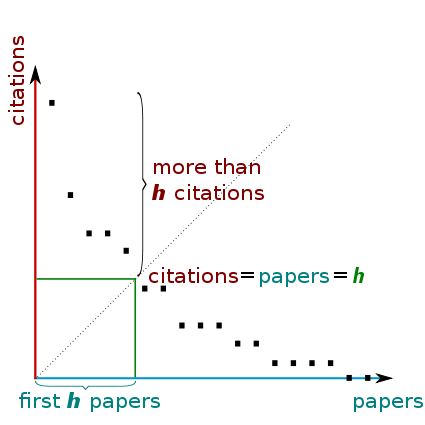
\epsfig{file=figures/hindex.eps}
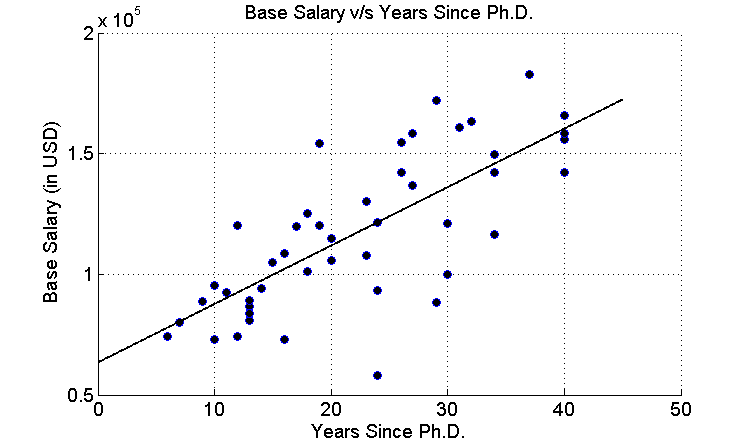
\includegraphics[width=0.5\textwidth]{figures/yrPhD.png}
\caption{Base salary plotted against years since Ph.D. shows a correlation.}
\end{figure}

This gives our generic simple linear regression model:

\begin{equation}
  \label{eqnourmodel}
  salary = \beta_0 + \beta_1 \text{Years Since Ph.D.} + \beta_2 \text{Productivity}
\end{equation}
